\documentclass{ctexart}
\begin{document}
\title{计算物理作业 13}
\author{刘畅, PB09203226}
\maketitle

{\bf [作业 13]}: 进行单中心 DLA 模型的模拟, 至少用两种方法算出相应图形的分形维数.

\bigbreak
单中心 DLA 模型的模拟第11次作业已经做过了, 这里直接把模拟的结果拿过来. 上次模拟的
结果是:
\begin{center}
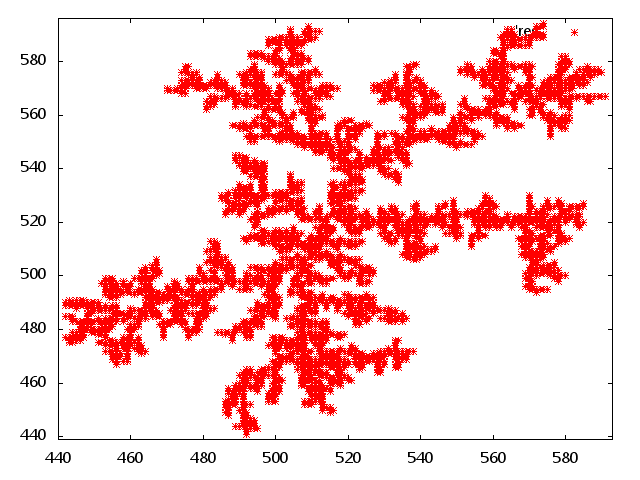
\includegraphics[width=3.5in]{dla.png}
\end{center}

为计算分形维数, 我们首先采用的算法是 sandbox 法. 这个算法计算以格点中心为中心,
长宽都为 $r$ 的矩形中 DLA 生长得到的粒子数 $N(r)$, 作出双对数曲线, 拟合得到的
斜率就是 DLA 图形的分形维数.

由于这个问题涉及的数据量太小并且涉及到比较多的输入输出, 用 C 语言编码就非常愚蠢了,
因为代码量大, 效率上的改进很小. 因此选择脚本语言 python. 代码见 \verb|frac_dim.py|.
这个问题改用 python 编程后, 核心的代码不过 20 行, 如果用 C 语言的话就远不止这个数了.

算法的主要部分是统计矩形内的粒子数:
\begin{verbatim}
def count_points_rect(data, w, x, y):
    npoints = 0
    for v in data:
        if -w <= v[0]-x <= w and -w <= v[1]-y <= w:
            npoints += 1
    return npoints
\end{verbatim}
接下来就只要对某个范围内的 \verb|w| (我选的是 1 到 70) 的调用上面的函数,
得出 $N(w)$, 再取双对数即可. (\verb|get_sandbox_dim()|)
\begin{verbatim}
for i in range(1, 70):
    f.write("%.12f %.12f\n" %
            (math.log(i), math.log(count_points(data, i, x, y))))
\end{verbatim}
从得到的数据文件作出图形:
\begin{center}
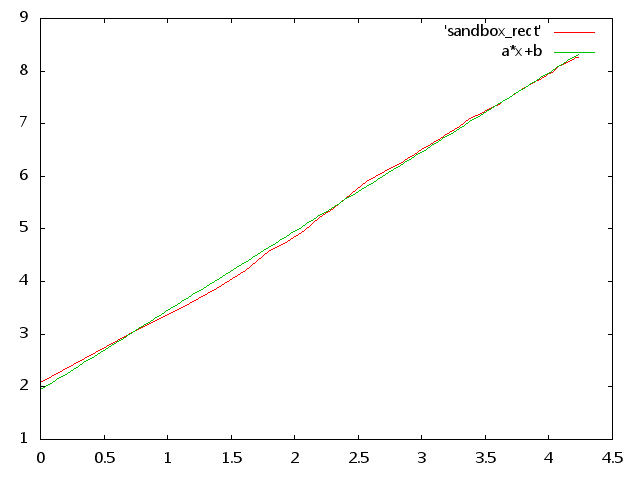
\includegraphics[width=4in]{sandbox_rect.png}
\end{center}
拟合出直线, 斜率就是要求的分形维数:
\[
d = \input sandbox_rect_res\relax
\]
我在文献上查到的结果是这个分形维数 $d=1.7$. 可以看到是基本一致的, 略微有一些偏差.
因此我考虑是否将矩形区域改为圆会对结果产生影响. 因为一维时有周长和半径的关系:
$l = 2\pi r$, 二维时有 $A = \pi r^2$, 三维时有 $V = \frac{4\pi}{3}r^3$.
因此推广到维数为 $d$ 应该有 $N(r)\propto r^d$. 取双对数后有 $\ln N(r) \sim
d\ln r$. 结果应该和前面的一致. 因此我们把上面的 \verb|count_points_rect()| 改成:
\begin{verbatim}
def count_points_circle(data, r, x, y):
    npoints = 0
    for v in data:
        if (v[0] - x)**2 + (v[1] - y)**2 < r**2:
            npoints += 1
    return npoints
\end{verbatim}
这个函数统计中心在 $(x,y)$ 半径为 $r$ 的圆内的粒子数. 其余代码不变, 得出的结果是:
\begin{center}
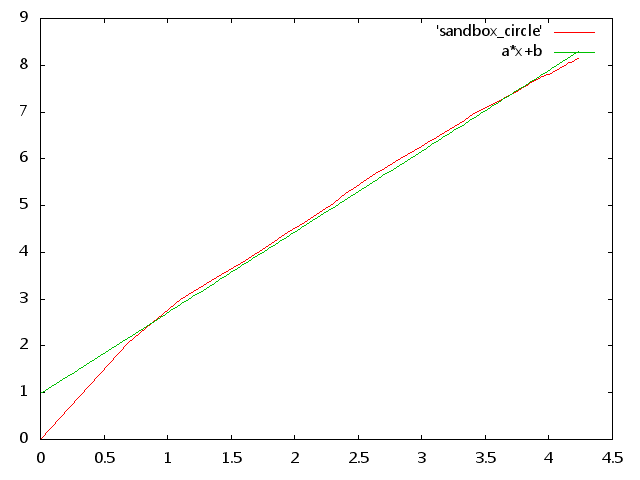
\includegraphics[width=4in]{sandbox_circle.png}
\end{center}
拟合直线得到的维数为:
\[
d = \input sandbox_circle_res\relax
\]
可以看到和文献上给出的值更加接近.

然后我们采用回转半径法来计算分形维数. 回转半径的定义是
\[
R_g = \sqrt{\frac{\sum_i r_i^2}{N}}
\]
其中的求和是对生长到某一阶段的 DLA cluster 取的. 在这个问题中, 我们取半径为
$r$ 的圆内的粒子求回转半径:
\begin{verbatim}
def get_radius_gyration(data, max_r, x, y):
    r_gy = 0.0
    npoints = 0
    for v in data:
        r2 = (v[0]-x)**2 + (v[1]-y)**2
        if r2 < max_r**2:
            r_gy += r2
            npoints += 1
    return npoints, math.sqrt(r_gy/npoints)
\end{verbatim}
上面的代码计算中心在 $(x,y)$ 半径为 \verb|max_r| 的圆内的粒子的回转半径.
返回值是这个圆内的粒子数和回转半径 (python 函数可以有多个返回值). 其余的代码和前面
一样, 就是作出双对数曲线并拟合直线求出斜率. 结果为
\begin{center}
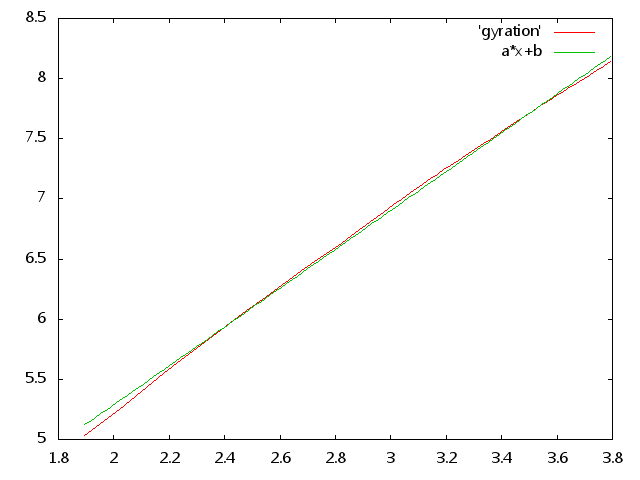
\includegraphics[width=4in]{gyration.png}
\end{center}
得到的分形维数为
\[
d = \input gyration_res\relax
\]
可以看到在前两个值之间.

\end{document}